\begin{document}	
\betterposter{
%%%%%%%% MAIN COLUMN

\maincolumn{
%%%% Main space

\textbf{We failed to detect a causal effect of FMD on CKD}. However, due to the \textbf{small number of relevant SNPs}, we had \textbf{limited power}. 
}{
%%%% Bottom space

%% QR code
\qrcode{img/qrcode}{img/smartphoneWhite}{
\textbf{Take a picture} to
\\download the full paper
}
% Smartphone icon
% Author: Freepik
% Retrieved from: https://www.flaticon.com/free-icon/smartphone_65680

%% Compact QR code (comment the previous command and uncomment this one to switch)
%\compactqrcode{img/qrcode}{
%\textbf{Take a picture} to
%\\download the full paper
%}

}

}{
%%%%%%%% LEFT COLUMN

\title{Assessing Evidence That Fibromuscular Dysplasia Causes Chronic Kidney Disease: A Two-Sample Mendelian Randomization Study}
\author{Frederick J. Boehm}
\author{Min-Lee Yang}
\author{Xiang Zhou}
\author{Santhi K. Ganesh}
\institution{University of Michigan}

\section{Introduction}
\textbf{Fibromuscular dysplasia (FMD)} is a systemic disease of artery walls that decreases target organ perfusion. 
Investigators have identified \textbf{chronic kidney disease (CKD)} as a possible consequence. 
% is there other evidence for this relationship? actual epidemiology studies??
% cite the actual case studies!!
\begin{center}
\includegraphics[width=\textwidth]{Fibromuscular.png}
\end{center}    

\begin{itemize} % perhaps add facts or evidence in itemized list below, to tie ckd to fmd
\item FMD often affects renal arteries \cite{olin2012united}.
\item FMD complications include stroke, dissection, \& aneurysm \cite{olin2012united}.
\end{itemize}

\section{Mendelian Randomization}


% https://media.springernature.com/full/springer-static/image/art%3A10.1038%2Fs41431-022-01038-5/MediaObjects/41431_2022_1038_Fig1_HTML.png?as=webp
    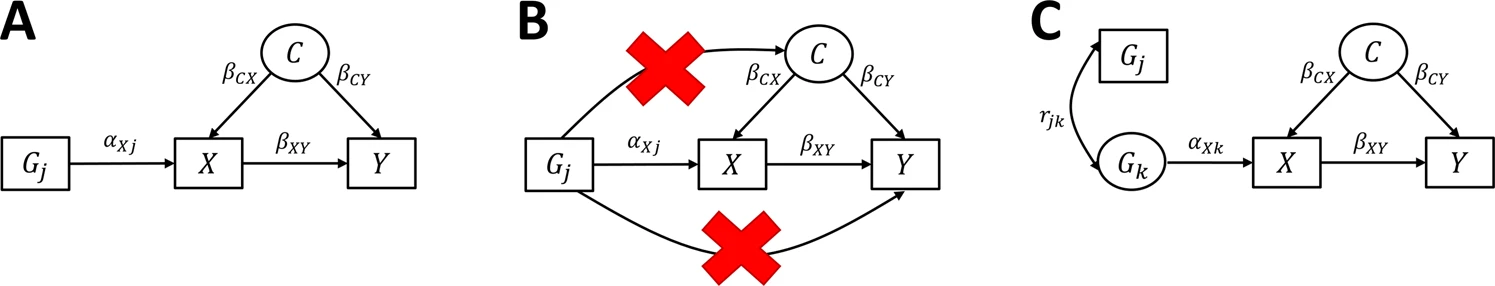
\includegraphics[width=\textwidth]{mr.png} % is this the figure that I want to use? 
    % Check the latest figures in teh Gen Epi letter about MR diagrams
    \cite{de2022understanding}




%% This fills the space between the content and the logo
\vfill

%% Institution logo

\includegraphics[width=\textwidth]{img/logo}\\

}{
%%%%%%%% RIGHT COLUMN
\section{Two-sample MR with GWAS Summary Statistics}
\begin{itemize}
\item FMD GWAS \cite{georges2021genetic}
\item CKD GWAS \cite{neale_lab_gwas}
\end{itemize}


\section{FMD GWAS Meta-analysis \cite{georges2021genetic}}
\begin{itemize}
\item Six case-control studies from USA and Europe  
\item 1556 cases \& 7100 controls  
\item Tested 5.5 million SNPs  
\item Identified four risk loci for FMD: \textit{PHACTR1, LRP1, LIMA1, ATP2B1}  
\end{itemize}
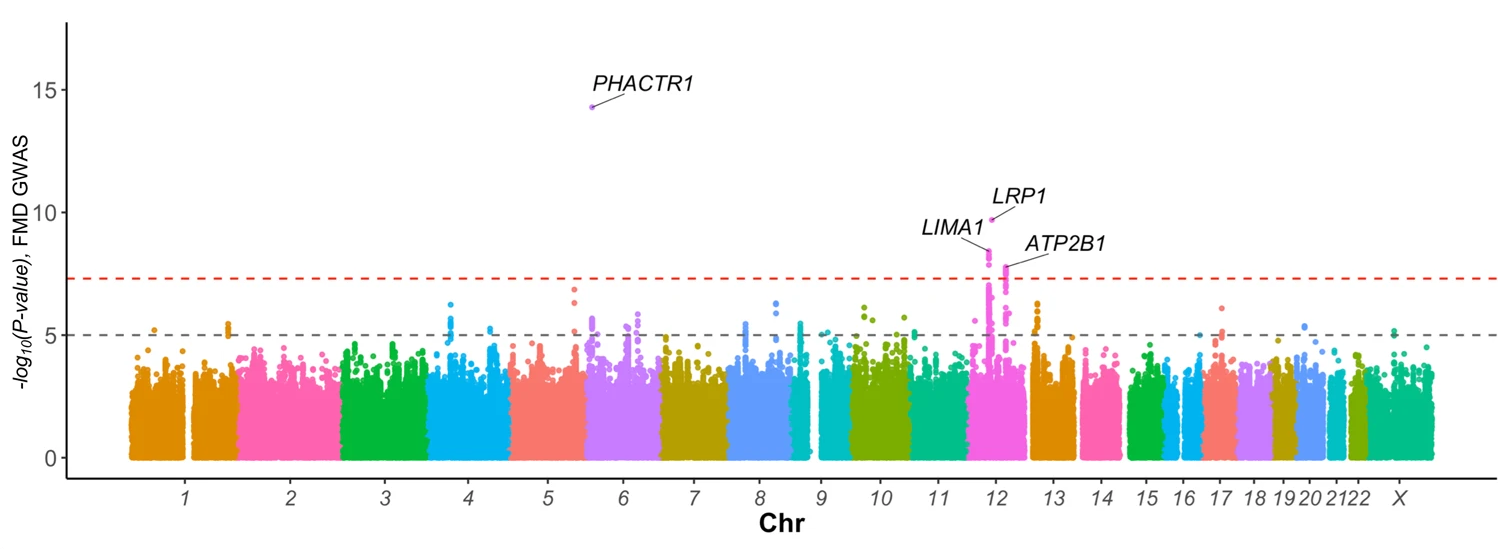
\includegraphics[width=\textwidth]{georges2021-Fig1.png} 




\section{CKD GWAS \cite{neale_lab_gwas}}
\begin{itemize}
\item 194,174 female UKB subjects -- check number of missing for this trait!
\end{itemize}


\section{MR Results}




\section{Conclusion}





\section{References}
\printbibliography[heading=none]


\section{Contact}
\textbf{Fred Boehm}\\
Email: frederick.boehm@gmail.com\\
Website: \url{https://fboehm.us}\\
Poster repository: \url{https://github.com/fboehm/statgen2024}


\section{Acknowledgements}
\textbf{Funding}: The National Institutes of Health (NIH) grant T32HL007853 to David J. Pinsky supported our research. The University of Michigan Postdoctoral Association supported our participation in STATGEN2024. 

}
\end{document}
